
\chapter{图像处理基本理论}

\section{图像增强}

实际图像不是完美的。由于噪声和光照等原因,图像的质量达不到自动识别的要求,所以需要进行图像增强\upcite{img_process}。图像增强可以突出待识别的目标的特征,抑制噪声和目标外的部分,从而使增强的图像更适合计算机识别。常见的图像增强方法有\emph{灰度变换}和\emph{图像平滑}。

\subsection{灰度变换}

灰度变换就是将图像每个像素的灰度变换成另一种灰度。灰度变换后每个像素的灰度仅仅由变换前的灰度决定。如果输入图像为$F(i,j)$,输出图像为$G(i,j)$,则灰度变换可以表示为:
\begin{equation}
  G(i,j)=T(F(i,j))
\end{equation}
变换函数$T(x)$可以由用户指定,也可以根据直方图确定。\emph{直方图均衡}就是一种根据直方图确定变换函数的方法。直方图均衡主要用于增加图像的全局对比度,改善光照条件不佳的图像。例如对背景或前景过亮或过暗的图像进行光照补偿,增强曝光过度或曝光不足的图像的细节等。直方图均衡化使输出图像包括所有可能的灰度级,并在每个灰度级上有大致相等的像素个数。要达到上述要求,首先求出直方图。设$n$表示图像的像素数,$n_i$表示灰度$i$出现的次数。灰度$i$有$0,1,\cdots,L-1$共$L$个灰度级。则直方图均衡化的灰度变换函数$T(x)$可以用如下方式求出。直方图$p(i)$表示灰度$i$出现的概率,用公式表示为:
\begin{equation}
  \label{eq:hist}
  p(i)=\frac{n_i}{n},i=0,1,\cdots,L-1
\end{equation}
再从直方图求出累计概率函数$c(i)$,定义如下:
\begin{equation}
  \label{eq:acc}
  c(i)=\sum_{j=0}^i p(j)
\end{equation}
最后将$c(i)$映射到$L$个灰度级:
\begin{equation}
  \label{eq:map}
  m(c(i))=\left[\frac{c(i)-\min(c(i))}{\max(c(i))-\min(c(i))}\cdot L\right]
\end{equation}
此时得到灰度变换函数为$T(x)=m(c(x))$。

\subsection{图像平滑滤波}

原始图像一般含有较多的噪声。噪声一般表现为盐椒噪声或孤立的点线噪声。图像平滑滤波使图像模糊化,取出极小的细节或将图像内的小间断连接起来。图像平滑滤波的基本方法是在像素的邻域内,对邻域内的像素和对应的系数的乘积求和。邻域内像素位置对应的权值一般用\emph{表示}。用模板进行图像滤波的方法如下:
\begin{asparaenum}[(1)]
\item 将模板中心与某个像素重合;
\item\label{enum:mul} 将模板上的权值和模板下对应的像素值相乘;
\item\label{enum:sum} 将第(\ref{enum:mul})所得的所有乘积相加;
\item 将模板中心的像素的灰度值用第(\ref{enum:sum})步的结果代替。
\end{asparaenum}


\emph{盒形滤波}是最简单的平滑滤波方法。它将每个像素的灰度用其邻域的算术平均值代替。设$F(i,j)$表示输入图像,$G(i,j)$表示平滑的图像,$S$表示邻域的像素坐标集合,$M$表示邻域的像素数目,则盒形滤波可以用公式表示为
\begin{equation}
  G(i,j)=\frac{1}{M}\sum_{(m,n)\in S}F(m,n)
\end{equation}
盒形滤波的模板如图\ref{fig:box}所示。
\begin{figure}[!h]
  \centering
  \includegraphics{box.eps}
  \caption{盒形滤波的模板}
  \label{fig:box}
\end{figure}

\emph{高斯滤波}也是一种常见的图像平滑滤波器。高斯滤波的模板对距离中心越远的位置,取越小的权值。与盒形滤波模板相比,高斯滤波更适合消除高斯噪声。这是因为空间域的高斯函数的傅立叶变换是频率域的另一个高斯函数,说明进行高斯滤波时,空间域内噪声对应的高频部分的衰减程度比低频部分大,噪声得到较大的抑制。高斯滤波对边缘的影响比盒形滤波小。这是因为图像的边缘中心像素和周围像素反差较大。应用盒形滤波时,由于模板对边缘中心和周围像素取相同的权值,边缘和周围区域的反差减小,不利于边缘检测。而对边缘应用高斯滤波时,模板中心的权值比周围像素的权值大,边缘和周围区域的反差减小的幅度较低,对边缘检测的影响较小。

为求出高斯滤波模板,需要定义高斯函数。标准差为$\sigma$的一元高斯函数定义为:
\begin{equation}
  \label{eq:gauss1}
  g(x)=\frac{1}{\sqrt{2\pi}\sigma}\exp\left\{-\frac{x^2}{2\sigma^2}\right\}
\end{equation}
将一元高斯函数绕$y$轴旋转,得到标准差为$\sigma$的二元高斯函数定义如下:
\begin{equation}
  \label{eq:gauss2}
  g(x,y)=\frac{1}{2\pi\sigma^2}\exp\left\{-\frac{x^2+y^2}{2\sigma^2}\right\}
\end{equation}

由式\eqref{eq:gauss2}可知,高斯滤波具有各向同性,即对任意方向都进行相同程度的平滑滤波。这一特性可以减小图像平滑对图像边缘的影响。因为边缘检测需要检测像素的梯度,如果对不同方向的平滑程度不同,则梯度的方向可能发生变化。

在二维高斯滤波函数的整点处进行采样,就得到高斯滤波的模板。高斯函数虽然在整个二维平面内都有定义,但在半径为$3\sigma$的邻域内的积分已达到0.99,即99\%的值包含在这个邻域内。因此模板只需覆盖半径为$3\sigma$的邻域就能达到滤波效果。设模板大小为$n\times n$,则$n$和标准差$\sigma$的关系为$n\approx 3\sigma+1$。在需要快速计算的场合,一般将模板内各点的高斯函数值数扩大若干倍再取整,得到权值均为整数的近似高斯模板,如图\ref{fig:gaussian}所示。
\begin{figure}[!h]
  \centering
  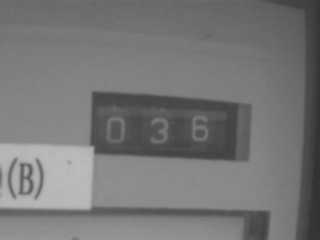
\includegraphics{gaussian.eps}
  \caption{$3\times 3$近似高斯模板}
  \label{fig:gaussian}
\end{figure}

直接计算模板较大的高斯滤波非常耗时。为了减少计算时间,可以利用二维高斯函数的可分离性。可分离性指二维高斯函数可以用两个一维高斯函数的乘积表示。由式\eqref{eq:gauss1}和式\eqref{eq:gauss2}可得:
\begin{equation}
  \label{eq:sep}
  \begin{array}{rl}
    g(x,y) &= \frac{1}{2\pi\sigma^2}\exp\left\{-\frac{x^2+y^2}{2\sigma^2}\right\} \\
    &= \frac{1}{\sqrt{2\pi}\sigma}\exp\left\{-\frac{x^2}{2\sigma^2}\right\}\frac{1}{\sqrt{2\pi}\sigma}\exp\left\{-\frac{y^2}{2\sigma^2}\right\} \\
    &g(x)g(y)
  \end{array}
\end{equation}
% \begin{enumerate}[(1)]
% \item 离模板中心越远的点,其权值逐渐减小到零。
% \item 总权值集中在$2\sigma$的范围内,故用标准差$\sigma$决定邻域的范围。
% \item 多个高斯滤波可以合并为一个高斯滤波过程。
% \item 对抑制高斯白噪声非常有效。
% \end{enumerate}

加权均值模板滤波的缺基本缺陷是抑制噪声和保留边缘的矛盾。模板越大,抑制噪声的效果越好,边缘也越模糊。但当模板处在两块区域的边缘时,由于两块区域的灰度差别很大,取加权平均值导致边缘处的灰度差别变小,不利于后续的边缘检测。即用模板中心权值较大的高斯滤波模板,边缘也有一定的失真。为了做到既能减少噪声,又能保持边缘,可以采用中值滤波。中值滤波就是用模板下所有像素灰度的中值代替原像素值。由于只需知道第$\frac{1}{2}(n-1)$大的像素值,不需要知道其他像素值的相对大小,可以巧妙地改造快速排序算法求出快速地求出中值。选取数组中的某个值,如果将分割点和$\frac{1}{2}(n-1)$比较,发现当分割点小于$\frac{1}{2}(n-1)$,说明中值包含在较大的数组中,当分割点大于$\frac{1}{2}(n-1)$时,说明中值包含在较小的数组中。这时只需对包含中值的数组递归地采用上述分割方法。

\section{边缘检测}

边缘是分割图像的一个重要特征。在灰度图像中,边缘表现为灰度有突然变化的区域。因此,边缘检测的经典算法是用每个像素所在邻域内的灰度变化确定边缘,而邻域内的灰度变化可以用邻域的导数刻画。这种利用利用邻域内的导数检测边缘,称为边缘检测局部算子法。

\subsection{一维信号边缘检测}

首先讨论一维信号的边缘检测算子,这不仅直观,也很容易推广到二维图像的边缘检测算子。而且一维信号的边缘检测算子也有实际用途,如用一维信号的边缘检测算子找出灰度直方图的波峰波谷。一维信号$f(x)$在邻域内的变化率用导数刻画:
\begin{equation}
  \label{eq:diff}
  \frac{\mathrm{d}f}{\mathrm{d}x}=\lim_{\Delta x\to 0}\frac{f(x+\Delta x)-f(x)}{\Delta x}
\end{equation}
连续信号$f(x)$无法直接观测,只能观测到间隔为1的离散信号$f(i)$,所以用差分$f'(i)=f(i+1)-f(i)$估计$f'(x)$。一阶差分相当于将模板$M'=[-1,1]$应用到一维信号中。模板$M'$的中心为左边的点。同理可得,$f(x)$的二阶导数可以用$f(i)$的二阶差分近似,相当于对$f(i)$应用模板$M''=[1,-2,1]$进行运算。

上述模板运算只利用了$i$和$i+1$处的值,和$i-1$没有关系。为了对称地利用$i$处的邻域,采用导数的对称的定义。
\begin{equation}
  \label{eq:diff2}
  \frac{\mathrm{d}f}{\mathrm{d}x}=\lim_{\Delta x\to 0}\frac{f(x+\Delta x)-f(x-\Delta x)}{2\Delta x}
\end{equation}
同样取$\Delta x=1$,得到一阶导数的近似值对应的模板为$M'_2=\frac{1}{2}[-1,0,1]$,二阶导数的近似值对应的模板为$M'_2=\frac{1}{2}[-1,-1,1,1]$。按照边缘处的一阶和二阶导数值分类,边缘可以分为阶跃形边缘、屋脊状边缘和斜坡形边缘。在阶跃形边缘处,一阶导数在此处存在一个脉冲,二阶导数在此处存在一个过零点。在屋脊状边缘处,一阶导数在此处存在阶跃,二阶导数在此处存在一个脉冲。在斜坡行边缘处,一阶导数在此处存在极值。如果发现导数存在这些特征,说明检测到边缘。

\subsection{二维图像边缘检测算子}

与一维图像的导数不同,二维图像的导数不仅有幅度,还有方向。图像$f(x,y)$可能在任意方向均存在导数。其中两个特殊的方向导数分别为沿着$x$和$y$轴方向的两个导数$f_x$和$f_y$,其他方向的导数都可以表示为这两个方向导数的线性组合。如果将$y$视为参量,则$f_x$可以视为以$x$为变量的一元函数,可以将模板$M'_2=[-1,0,1]$应用于$f(x,y)$求出该导数的近似值。然而,由于图像含有噪声,而且边缘不一定沿$x$方向,因此应该将模板应用于像素本身及其上下两个相邻像素,求出三个近似值,再求出这三个近似值的平均值作为该处$f_x$的估计值。这个计算过程相当于将如图\ref{fig:prewitt_x}所示的模板应用于图像$f(x,y)$。同理可得计算$f_y$的模板,如图\ref{fig:prewitt_y}所示。
\begin{figure}[!h]
  \centering
  \subfloat[x方向]{\label{fig:prewitt_x}\includegraphics{prewitt_x.eps}}\hspace{1cm}
  \subfloat[y方向]{\label{fig:prewitt_y}\includegraphics{prewitt_y.eps}}
  \caption{Prewitt算子}
\end{figure}
一种类似的算子是Sobel算子,如图\ref{fig:sobel}所示,它对中间一行运算的权值是上下两行的权值的两倍。
\begin{figure}[!h]
  \centering
  \subfloat[x方向]{\includegraphics{sobel_x.eps}}\hspace{1cm}
  \subfloat[y方向]{\includegraphics{sobel_y.eps}}
  \caption{Sobel算子}
  \label{fig:sobel}
\end{figure}

根据二元函数微分学,二维图像$f(x,y)$沿\emph{梯度}方向灰度变化最大。图像的梯度定义为向量$\nabla f=(f_x,f_y)$,梯度的幅值为$|\nabla f|=\sqrt{f_x^2+f_y^2}$,方向为$0=\arctan\left(\frac{f_y}{f_x}\right)$。为了减少计算量,梯度幅值一般简化为计算$\frac{1}{2}(f_x^2+f_y^2)$或$\max(|f_x|,|f_y|)$或$|f_x|+|f_y|$。另一种简化计算梯度的方法是利用与标准行列方向偏离45度的两个交叉的差分作为方向导数。这两个方向导数在$(i,j)$处的估计值为$f(i+1,j+1)-f(i,j)$和$f(i,j+1)-f(i,j+1)$。这两个差分运算可以用图\ref{fig:robert}所示的模板表示,称为Roberts算子。用上述算子求出梯度和幅值后,追踪具有高幅值的点,或追踪幅度极值点,可以得到边缘。
\begin{figure}[!h]
  \centering
  \subfloat{\includegraphics{robert_x.eps}}\hspace{1cm}
  \subfloat{\includegraphics{robert_y.eps}}
  \caption{Robert算子}
  \label{fig:robert}
\end{figure}

上述边缘算子的基本缺陷就是检测精度和抗噪声能力不能兼顾。由于图像的边缘和噪声均为灰度急剧变化的部分,简单的梯度运算会将噪声误认为边缘。Canny应用严格的数学方法分析边缘检测的缺陷,并提出平衡检测精度和抗噪声能力的方法。Canny给出了评价边缘检测的三个准则:
\begin{enumerate}[(1)]
\item 信噪比准则:信噪比越大,边缘质量越高。
\item  定位精度准则,即检测出的边缘点尽量靠近实际边缘。
\item 单边缘响应准则:即单个边缘只产生一个响应,虚假边缘响应得到最大抑制。
\end{enumerate}

为满足上述准则,Canny利用最优化方法,得到了最佳边缘模板。Canny针对一维边缘,推导出的最优边缘检测算子与高斯函数的导数类似。在实际应用中,为了减少计算量,可以用高斯滤波后再用Sobel算子求出方向导数的幅度和方向,用于近似计算Canny的最优边缘检测算子。

此时得到原始图像的梯度图像。梯度较大处都是边缘的候选点。但一个真实的边缘点附近往往有许多虚假的边缘响应,在图像中表现为一条较粗的边缘。为了细化边缘,在邻域内的多个边缘响应点只用保留一个。通过判断候选点是否为其梯度方向上的邻域的极大值判定该点是否为边缘点。具体做法是,对某个候选点,在其梯度方向上找出一个邻点,要求该邻点和候选点的连线与梯度方向相差不到45度。然后再其梯度的反方向上满足同样要求的邻点。比较候选点和这两个邻点的梯度幅值,如果候选点的梯度幅值高于两个邻点,则保留该候选点,否则删除该候选点。这一过程称为\emph{非极大值抑制},如算法\ref{alg:nms}所示。
% \begin{algorithm}[H]
%   \caption{非极大值抑制}
% \label{alg:nms}
% \begin{algorithmic}
%   \REQUIRE $\textrm{梯度幅值图像}M\textrm{和梯度方向图像}D$
% \ENSURE $\textrm{边缘细化的梯度图像}N$
% \FOR {$i\gets 0$ \TO $\max(i)$}
% \FOR {$j\gets 0$ \TO $\max(j)$}
% \STATE $N_1[4]\gets\{(1,0),(1,1),(0,1),(-1,1)\}$
% \STATE $N_2[4]\gets\{(-1,0),(-1,-1),(0,-1),(1,-1)\}$
% \STATE $d\gets D(i,j) \mod \frac{\pi}{4}$
% \STATE $(u_1,v_1)\gets (i,j)+N_1[d]$
% \STATE $(u_2,v_2)\gets (i,j)+N_2[d]$
% \IF {$M(i,j) > M(u_1,v_1)$ \AND $(M(i,j) > M(u_2,v_2)$}
% \STATE $N(i,j)\gets M(i,j)$
% \ELSE
% \STATE $N(i,j)\gets 0$
% \ENDIF
% \ENDFOR
% \ENDFOR
% \end{algorithmic}
% \end{algorithm}

过极大值抑制后,边缘仅为单像素宽。然而这些边缘仍然存在虚假边缘响应点。使用双阈值的方法提高边缘质量。选取高低两个阈值。在梯度图像中找出幅度高出高阈值的点。,然后将这些邻点作为新的起点,再找出它们周围高于低阈值的邻点。

\section{图像分割}

图像分割就是将图像划分成多个区域,这些区域内的特征表现相似,而不同区域间特征显著不同。常见的特征有灰度、色彩、纹理和几何形状。图像分割的有两个目的。第一个目的是分离目标和背景,为图像识别奠定基础。第二个目的将像素组织成更高级的单元,进而从区域的角度而不是像素的角度更好地分析图像。
目前没有一种通用的分割方法,适用于各个领域,需要根据具体情况选择合适的分割算法。

\subsection{阈值分割}


\subsection{轮廓分割}

\section{二值图像分析}

图像分割后的结果一般是二值图像,其中目标像素值设为1。背景像素值设为0。在文档扫描和工业机器视觉系统中,计算机系统都是以二值图像作为识别的对象。二值图像算法的应用场合十分广泛,例如目标计数、定位和识别等。

\subsection{连通成分标记}

\emph{连通成分}指具有相同的灰度且其中任意像素都有相邻像素的像素集合。连通成分标记就是用不同的标号区分不同的连通成分,每个连通成分的像素值设定为其所在的连通成分的标号。标记连通成分有两种基本算法:\emph{递归搜索算法}和\emph{逐行扫描算法}。

递归搜索算法的基本思想是将某个具有最大灰度的像素作为种子像素,将其像素值设定为连通成分的标号。再从其相邻的像素中找出未标记且值为1的像素,将这些像素作为新的种子像素,递归地施行上述方法,直到标记完连通成分的所有像素。然后找出另一连通成分的种子像素,施行同样的方法,直至标记出所有的连通成分。设$B$表示二值图像,$LB$表示连通成分的标记图像,$LB(i,j)$的初值为0,则算法如\ref{alg:comp}所示。
\begin{algorithm}[H]
  \caption{标记二值图像的连通成分}
  \label{alg:comp}
  \begin{algorithmic}
    \REQUIRE $\textrm{二值图像}B$
    \ENSURE $\textrm{连通成分标记}LB$
    \STATE $label\gets 0$
    \FOR{$i\gets 0$ \TO $M-1$}
    \FOR{$j\gets 0$ \TO $N-1$}
    \IF{$B(i,j)=1$ \AND $LB(i,j)=0$}
    \STATE $label\gets label+1$
    \STATE $\search(i,j,label)$
    \ENDIF
    \ENDFOR
    \ENDFOR
    \STATE $\textbf{procedure}\ \search(i,j,label)$
    \STATE $LB(i,j)\gets label$
    \STATE $N\gets \neighbours(i,j)$
    \FOR{$(i',j')\in N$}
    \IF{$B(i',j')=1$ \AND $LB(i',j')=0$}
    \STATE $\search(i',j',label)$
    \ENDIF
    \ENDFOR
  \end{algorithmic}
\end{algorithm}

在递归扫描算法中,每扫描一个像素就要做一次递归。数字图像的像素点很多,递归深度非常大,因此算法的时间和空间开销非常大。有人提出了逐行扫描算法,只需扫描图像两次。该算法扫描图像时,找出未标记的像素作为种子像素,设定其临时标号,将种子像素的临时标号传播到后续像素。由于种子像素的标号只能向右下转播,故其左下方也可能存在另一个种子像素\footnote{种子像素$P$的右上方也有可能存在种子像素$Q$。在这种情况下,我们将像素$Q$当作“当前”像素,则$P$仍然是“左下方”的像素。左上方的种子像素和“当前”种子像素不可能在同一个连通成分内,否则左上方的种子像素会将标号传播到“当前”种子像素,此时“当前”像素不是种子像素。所以只用考虑合并“当前”像素及其左下方像素的传播区域。}两个种子像素的标号可能传播到同一区域。如果出现这种情况,说明两个种子像素传播的区域在同一个连通成分内,应合并这两个区域,也就是将两个种子像素传播的区域改成相同的标号。因此需要再次扫描图像,合并上述区域。

\subsection{形态学运算}
%%% Local Variables: 
%%% mode: latex
%%% TeX-master: "thesis"
%%% End: 
